\documentclass{article}

\usepackage[final]{neurips_2019}
\usepackage[utf8]{inputenc}
\usepackage[T1]{fontenc}
\usepackage{amsfonts}
\usepackage{amsmath}
\usepackage{booktabs}
\usepackage[capposition=top]{floatrow}
\usepackage{graphicx}
\usepackage{hyperref}
\usepackage{microtype}
\usepackage{multirow}
\usepackage{nicefrac}
\usepackage{lipsum}
\usepackage{url}
\usepackage{xcolor}

\newcommand{\note}[1]{\textcolor{blue}{{#1}}}

\newcommand{\SubItem}[1]{
    {\setlength\itemindent{15pt} \item[-] #1}
}

\title{
  Face Mask Detection Using Machine Learning Models\\
  \vspace{1em}
  \small{\normalfont Stanford CS229 Final Project}\\
  \small{\normalfont Category: Computer Vision}\\
  \small{\normalfont November 18th, 2020}
}

\author{
  Charles Pan \\
  \href{mailto:cpan22@stanford.edu}{\texttt{cpan22@stanford.edu}} \\
  Stanford University \\
  \And
  Gilbert Rosal \\
  \href{mailto:rosalg@stanford.edu}{\texttt{rosalg@stanford.edu}} \\
  Stanford University \\
  \And
  Dean Stratakos \\
  \href{mailto:dstratak@stanford.edu}{\texttt{dstratak@stanford.edu}} \\
  Stanford University \\
}

\begin{document}

\maketitle

\section{Introduction}
Across the globe, there have been 55.6M million reported coronavirus cases (up from 33.8M last month). Covid-19 has plunged countless nations into chaos and recession as they scramble to keep the virus contained. Due to the highly contagious nature of the virus, every individual must do their part in preventing the spread by taking precautions such as wearing a face mask. Yet there are still many individuals who refuse to do so - this careless behavior puts many lives at risk, so it is imperative that we hold these individuals responsible.

In light of this issue, our project aims to create a machine learning model that can accurately detect, given an image, whether a person is properly wearing a face mask or not. This project will especially be important in the global return to work effort as businesses continue to search for ways to keep their employees and customers safe. Automating the process of face mask detection will reduce human labor while creating a system of accountability.

\section{Related Work}
Given the recency of COVID-19 pandemic, there hasn’t been too much existing research on face mask detection, but one recent study \cite{LOEY2021108288} has shown that machine learning models are definitely capable of achieving high performance with regards to this task. Their use of a hybrid model and use of ResNet50 for data extraction were extremely clever as they allowed for greater expressivity and powerful features that lended themselves to better predictions. Furthermore, the use of an SVM for the second part of their hybrid was incredibly smart since there are 3 discrete groups to identify in the data. The major drawback of their implementation is its runtime. This approach is state-of-the-art when it comes to mask recognition specifically, succeeding close to 99.5-100\% on experimental test sets.

In “Food Detection and Recognition Using Convolutional Neural Network”\cite{10.1145/2647868.2654970}, “Face Recognition: a Convolutional Neural-Network Approach”\cite{554195}, and “ImageNet classification with deep convolutional neural networks”\cite{10.1145/3065386}, they too use a CNN to classify pictures of food. As explained by Samer Hijazi in “Using Convolutional Neural Networks for Image Recognition”\cite{Hijazi2015UsingCN}, CNN’s strengths lie in their ability to withstand distortions to images, minimize memory usage, and undergo better training than convolution NN counterparts. This is because of CNN’s property of convolution at every layer, making it so the number of computations decreases as the layer number increases. This also reduces noise since there are less parameters to worry about compared to a standard NN.

Jianlong Fu et al. \cite{Fu_2017_CVPR} approach the problem of Fine-grained Image Recognition (like identifying whether something was a bird, but what species of bird it was) by creating a recurrent attention CNN (RA-CNN), which “recursively learns discriminative region attention and region-based feature representation in a mutually reinforced manner” since the two are correlated. At a high level, the RA-CNN cleverly uses a classification sub-network and attention proposal sub-network to find regions of images that can allow for image identification. From there the recurrent network optimizes, producing higher confidence scores with each step. This approach is strong in its expressiveness and accuracy, maintaining a 92.5\% success rate without labels. One considerable weakness is the models inability to model local visual cues, hindering performance at finer scales.

\section{Dataset and Features}
We obtained our face mask dataset from \href{https://www.kaggle.com/andrewmvd/face-mask-detection}{Kaggle}\cite{dataset}. This dataset contains about 853 images of people as the input and labels for each person in the image corresponding to wearing a mask, not wearing a mask, and wearing a mask incorrectly, as well as bounding boxes around the faces of people in the image. Each image contained a variable number of people, meaning one image could give us multiple data points.

To preprocess the data, we parsed the .xml file for the label and bounding box for any given face, extracted the image, then saved the label in a .csv file. We then normalized all images to a resolution of 64x64. This preprocessing got us from 853 images to 4072 images, but this still wasn’t enough. As a result, we implemented various data augmentation techniques including rotating, adding noise, flipping horizontally and vertically, gray scaling, changing contrast, gamma correcting, log correcting, sigmoid correcting, blurring, and shearing the images. We additionally normalized our images to a resolution of 64x64, and used each image’s pixel RGB values converted to grayscale to train our machine.

\begin{center}
  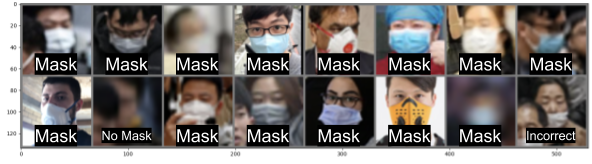
\includegraphics[width=4in]{../images/data.png}
\end{center}

\section{Methods}
The Face Mask Detection problem is a multinomial classification problem, where the output is discrete and one of correctly wearing a mask, incorrectly wearing a mask, and not wearing a mask at all. Given this, we implemented the following baselines:
\begin{enumerate}
  \item Multinomial Logistic Regression Model
  \item Support Vector Machine with Linear Kernel
  \item Support Vector Machine with RBF Kernel
  \item Support Vector Machine with Polynomial Kernel  
\end{enumerate}

To implement the softmax regression model, one must first express the multinomial distribution as a member of the exponential family. From here, the goal is to express $p(y=i|x;\theta)$. Using the link function of $\Phi_k = \sum_{j=1}^k \exp(\eta_i) = 1$, we derive
\begin{align*}
  \Phi_i = \frac{\exp(\eta_i)}{\sum_{j=1}^k \exp(\eta_j)},
\end{align*}
where $\Phi_i = p(y=1;\Phi)$ and $p(y=k;\Phi) = 1 - \sum_{i=1}^{k-1}\Phi_i$. Finally, because exponential families assume $\eta_i = \theta_i^\top x$, we can express
\begin{align*}
  p(y=i|x;\theta) = \Phi_i = \frac{\exp(\theta_i^\top x)}{\sum_{j=1}^k \exp(\theta_j^\top x)}.
\end{align*}

We use this expression to derive the probability a given data point lies in a given class. To optimize, softmax regression simply computes the theta that maximizes the log-likelihood through gradient descent or Newton’s method (from Lecture Notes 1, Section 9.2).

We believed SVMs would be an effective algorithm to train on because we're trying to take our dataset and divide it into different categories, with each category hopefully showing patterns of being grouped together such that decision boundaries can be drawn. Conceptually, SVMs determine a line that can divide the provided data based on whichever class the data is in; we call this line the decision boundary. The decision boundary determines the class of new data points based on whichever side of the decision boundary it's on. The decision boundary is determined by calculating the optimal margin, or the shortest distance between the observations and the decision boundary. We use kernels to transform data into higher dimensions, and the kernel trick ensures we never have to actually transform our initial data into higher dimensions (but we can still calculate the value as if it was in that higher dimension). We compute the optimal margin classifier (the decision boundary) by using the following expression:
\begin{align*}
  \min_{w,b} \frac{1}{2}\|w\|^2, \quad \text{s.t. } y^{(i)}(w^\top x^{(i)} + b) \geq 1 \quad \forall i \in {1, \dots, n},
\end{align*}
where $w$ and $b$ are the weights and bias, respectively, and $(x^{(i)}, y^{(i)})$ is the $i^\text{th}$ data point (Lecture Notes 3, Part IV).

After implementing these baselines, we decided to implement a convolutional neural network for our multiclass image classification problem as CNNs have been shown to be effective in tackling computer vision tasks. Specifically, we decided to use the ResNet50 CNN architecture after reading about successful results that another group of researchers had in a similar project when using ResNet50 \cite{he2015deep}. The ResNet50 architecture consists of a stack of convolutional, batchnorm, and ReLU layers as well as “identity” blocks with a final fully connected layer at the end.

We implemented two versions: one pure ResNet50 model initialized with empty weights and one pretrained ResNet50 model (initialized with weights learned from ImageNet) fine-tuned for our classification problem. We trained both using an Adam optimizer (default initialized with a 0.01 learning rate) and categorical cross entropy loss function. For the pure model, we trained the entire model over thirty epochs, while for the pretrained model, we fine tuned the final fully-connected layer over twenty epochs, and then the entire model over another ten epochs.


\section{Experiments, Results, and Discussion}
We split our dataset with 80\% training, 10\% validation, and 10\% testing. For the baselines, each image was first converted into a one dimensional array containing all the images’ pixels and then passed into the corresponding baseline. However, we noticed that our dataset was highly imbalanced with approximately 80\% of the images consisting of people wearing masks, 18\% not wearing masks, and 2\% wearing masks incorrectly, so we ended up upsampling two of our image classes. The final distribution consisted of 40\% of our images of people wearing masks, 40\% not wearing masks, and 20\% wearing masks incorrectly. We then fitted our models and calculated our results according to various metrics: raw/balanced score, confusion matrices, and ROC AUC scores, and the results are shown below in Table \ref{tab:table1} and Figure \ref{fig:figure1}.

\begin{table}[h!]
\begin{center}
\caption{Model comparison}
\label{tab:table1}
\bgroup
\def\arraystretch{1.5}
\begin{tabular}{llccc}
  \hline
                                                              &                     & Raw        & Balanced   & ROC AUC Average \\ \hline \hline
                                                              & Logistic Regression & 0.72094926 & 0.42041754 & 0.81690826      \\ \hline
  \multicolumn{1}{c}{\multirow{3}{*}{SVM}} & Linear              & 0.71522094 & 0.52980470 & 0.90478115      \\
  \multicolumn{1}{c}{}                                        & RBF                 & 0.88788870 & 0.54039438 & 0.80430017      \\
  \multicolumn{1}{c}{}                                        & Polynomial          & 0.83387888 & 0.42728988 & 0.93612327      \\ \hline
  \multirow{2}{*}{ResNet50}                                   & Pure                & 0.90600001 & 0.30808688 & 0.46376876      \\
                                                              & Pretrained          & 0.76800000 & 0.32577636 & 0.51320445      \\ \hline \hline
  \end{tabular}
\egroup
\end{center}
\end{table}

\begin{figure}[htp]
\caption{Confusion matrices}
\floatfoot{Note that 0 represents No Mask, 1 represents Mask, and 2 represents Incorrect Mask}
\label{fig:figure1}
\centering
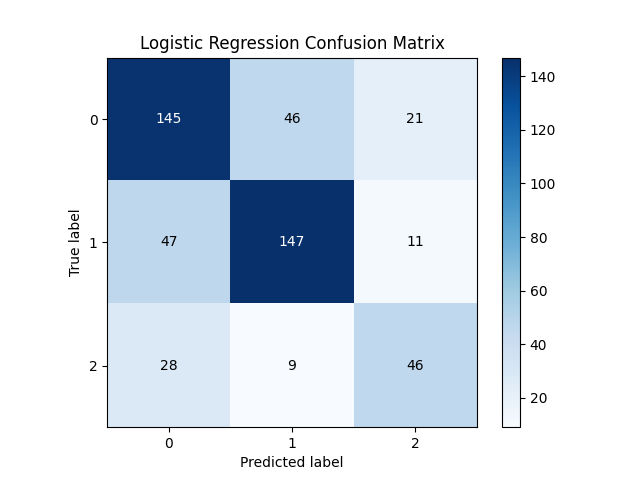
\includegraphics[width=.5\textwidth]{../results/logreg/confusion_matrix.png}\hfill
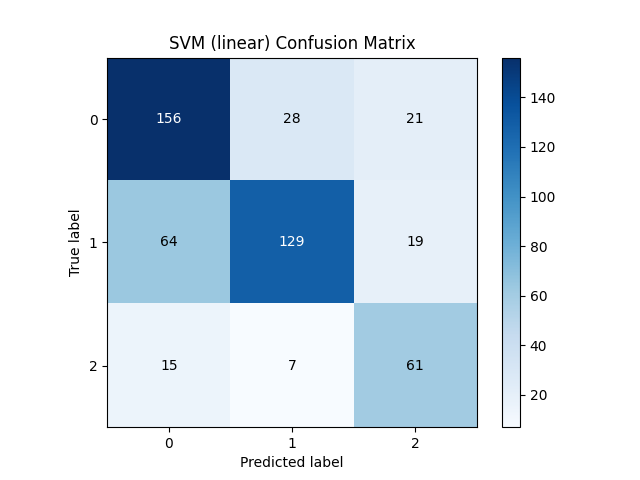
\includegraphics[width=.5\textwidth]{../results/svm/linear/confusion_matrix.png}\hfill
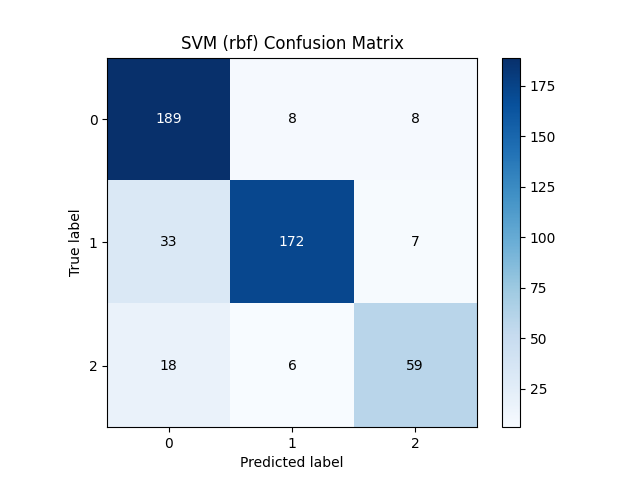
\includegraphics[width=.5\textwidth]{../results/svm/rbf/confusion_matrix.png}\hfill
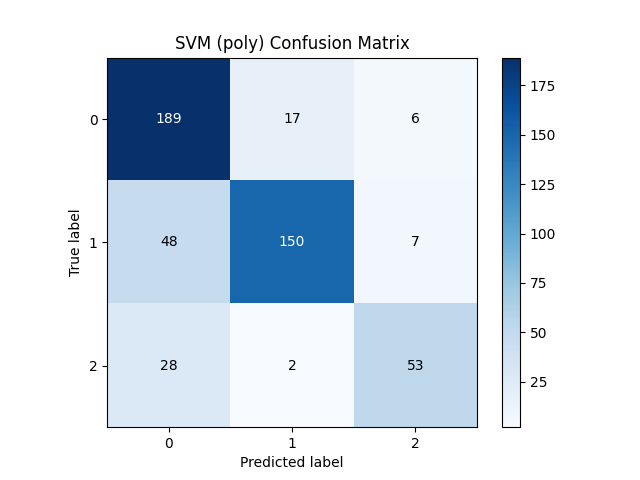
\includegraphics[width=.5\textwidth]{../results/svm/poly/confusion_matrix.png}\hfill
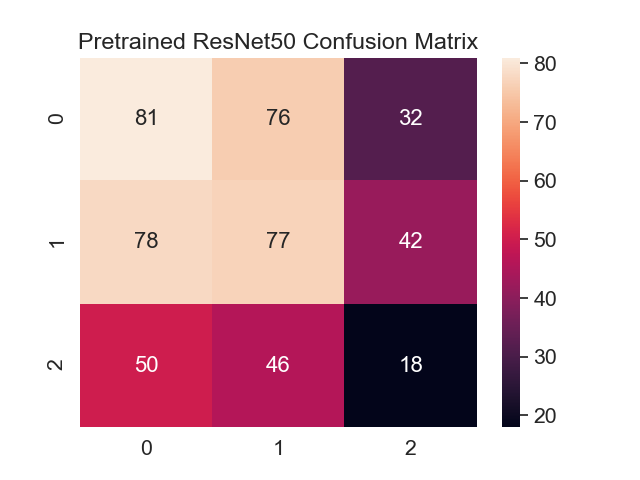
\includegraphics[width=.5\textwidth]{../results/resnet50/pretrained/confusion_matrix.png}\hfill

\end{figure}

Of the baselines, the support vector machine with RBF kernel performed by far the best. Interestingly, the pure ResNet50 model outperformed the pretrained ResNet50 model in terms of raw score, but the pretrained model did better in terms of balanced score and ROC AUC average score. This could be because the pure ResNet50 model was able to overfit significantly more than the pretrained model due to starting with empty weights. However, both these models underperform compared to the SVM linear and RBF models in all metrics except raw score.

In terms of qualitative results, we noticed that our ResNet50 models did relatively poorly in predicting incorrect wearing of masks. This seems to be backed up by our confusion matrix results showing exactly this. This could be because our models weren’t exposed to nearly enough incorrect samples to learn its features, as it was the least represented class.

In all, it is still a bit of a mystery to us as to why our ResNet model did not perform too well, especially when the other study achieved great results with it - we suspect that it is likely because our 4000 image training set was still too small to achieve any meaningful learning in our model. With more time, we would try more hyperparameter tuning with different learning rates, epochs, dropout rates, and data augmentation techniques. It also appeared that we ran into the exploding gradient problem during training, and in the future we likely will implement gradient clipping in order to prevent this.

\section{Conclusion}
In the era of COVID-19 and social distancing, an effective face mask detection system may be the key for getting employees back to work safely. In this project, we implemented various ML models to be able to determine if someone is correctly wearing a mask. From our experiments, a support vector machine with RBF kernel was shown to be the most effective through balanced score, confusion matrix, and ROC AUC average score. However, we suspect that in practice, the pretrained ResNet50 model would likely perform the best and only unperformed in our experiments due to a small training set size. With more time and more resources, we envision this model to be part of a larger ML pipeline implemented at the entrance of workplaces where the input is a live-stream video, and the pipeline can verify employee mask wearing as well as identify any number of faces at a single time.

\section{GitHub Link to Project}
\href{https://github.com/dastratakos/Face-Mask-Detection}{https://github.com/dastratakos/Face-Mask-Detection}

\section{Team Member Contributions}
Charles Pan
\begin{itemize}
  \item Implemented scikit-learn Logistic Regression and SVM baselines for each kernel and produced baseline results
  \item Implemented ResNet50 keras implementation and carried out training on GCP VM
  \item Implemented metrics calculation and reporting
\end{itemize}

Gilbert Rosal
\begin{itemize}
  \item Implemented first run Logistic Regression
  \item Helped implement data preprocessing such that models could interpret the images
  \item Worked on the project proposal and milestone write up
  \item Implemented function to divide images into folders based on class label
  \item Wrote introduction, related work, methods, dataset/features of write up
\end{itemize}

Dean Stratakos
\begin{itemize}
  \item Implemented the data preprocessing steps to digest .png images + .xml annotations and extract faces from images.
    \SubItem{Created data augmentation techniques.}
    \SubItem{Wrote visualization tool to draw bounding boxes.}
  \item Added CLI (command line interface) support for easy use.
  \item Worked on the project proposal, milestone, and final write up.
  \item Calculated metrics for baselines.
\end{itemize}

\bibliographystyle{unsrt}
\bibliography{references}

\end{document}
